\section{Scenario 1 - Angle Range}\label{sec:scenario1}
The first scenario describes the movement of a UA when it flies far away from the GS between two predefined positions (Figure \ref{fig:s1_map_a}). The distance between the aircraft and the GS can be represented by a parabola, as is described in Figure \ref{fig:s1_map_b}. In the beginning, the distance between both devices is around 48km and, while the UA is flying, the distance becomes smaller, achieving a minimum value. After this minimum, the distance between the devices increases until the UA reach the final position.

Based on Figures \ref{fig:s1_pd_gs_alone} and \ref{fig:s1_pd_ua_alone}, it is possible to observe that the azimuth and elevation angles of the UA and the GS often have different behaviours during the whole movement. 
  

\begin{figure}[H]
	\hfill
	\subfigure[UAS Map Positioning]{\label{fig:s1_map_a} 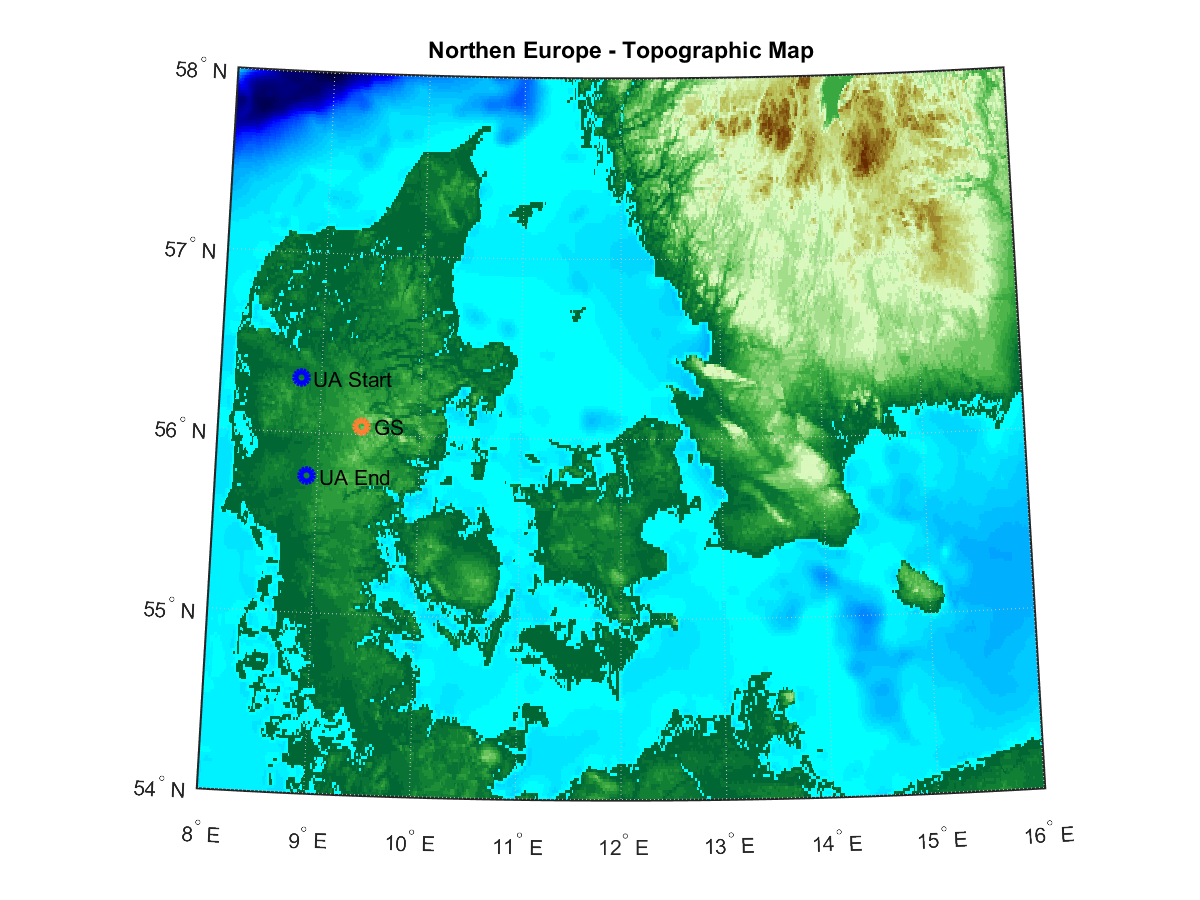
\includegraphics[scale=0.32]{figures/s1_map.png}}
	\hfill
	\subfigure[LOS and Distance]{\label{fig:s1_map_b} 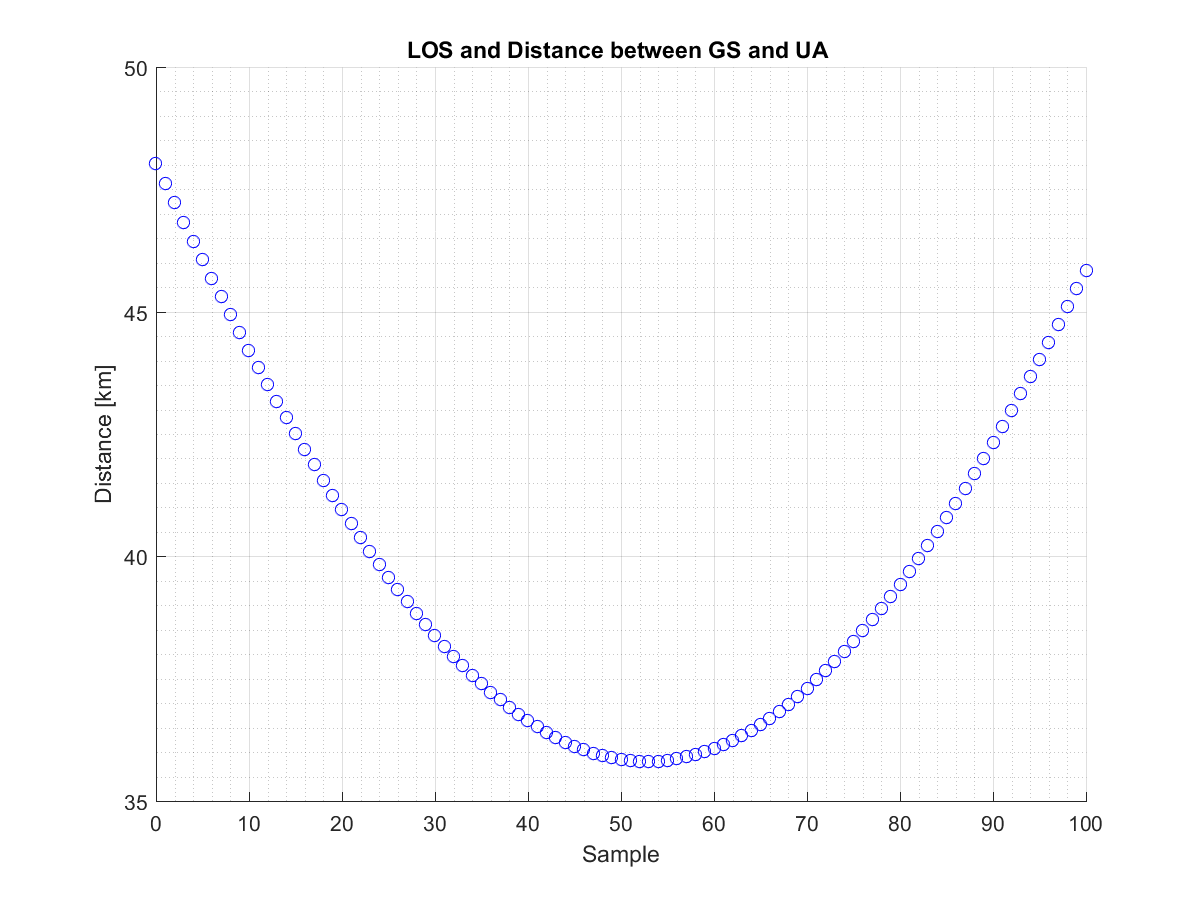
\includegraphics[scale=0.34]{figures/s1_los.png}}
	\hfill
	\caption{Angle Range Scenario}
	\label{fig:s1_map}
\end{figure}

\subsection{Ground Station}\label{GroundStation_scenario1}
As expected, the absolute value of the $\theta_{OPTIMAL}$ increases until it reaches 180$^{\circ}$  and, then, it starts increasing from -180$^{\circ}$ until the end. The initial $\theta_{OPTIMAL}$ is around 140$^{\circ}$ due to the system of coordinates applied where the Local NED frame coincides with the body frame. This assumption was taken into account because the position of the GS is static.

In the beginning, the amplitude of the azimuth angle is positive and is growing because the UA is flying on the left side of the GS (lower longitude) to south (decreasing latitude). However, there is a jump when $\theta$ reaches 180$^{\circ}$ in the first graph of Figure \ref{fig:s1_pd_gs_alone}. This happens due to the used convention which limits the range from -180 to 180$^{\circ}$. Nonetheless, there is a continuous rotation, which means that when the antenna achieves 180$^{\circ}$, it will continue rotate in the same direction starting from -180$^{\circ}$. Thus, after the jump, the amplitude of the azimuth angle will continue increase from -180 until -136$^{\circ}$.

On the other hand, the optimal elevation angle, $\phi_{OPTIMAL}$, has always a small amplitude because of the big distance between the UA and the GS of the second graph of Figure \ref{fig:s1_pd_gs_alone}. Since the previous distance is always bigger than 36km, a considerable optimal phi is not required to point at the UA. 

Despite of the small amplitude, $\phi_{OPTIMAL}$ has a maximum value (approximately 0.06$^{\circ}$) which corresponds to the minimum distance between the UA and the GS (closest point). Therefore, when the UA is closer, GS’s antenna needs to increase the angle in order to be able to continue pointing at the antenna in the aircraft.

\begin{figure}[H]
	\centering
	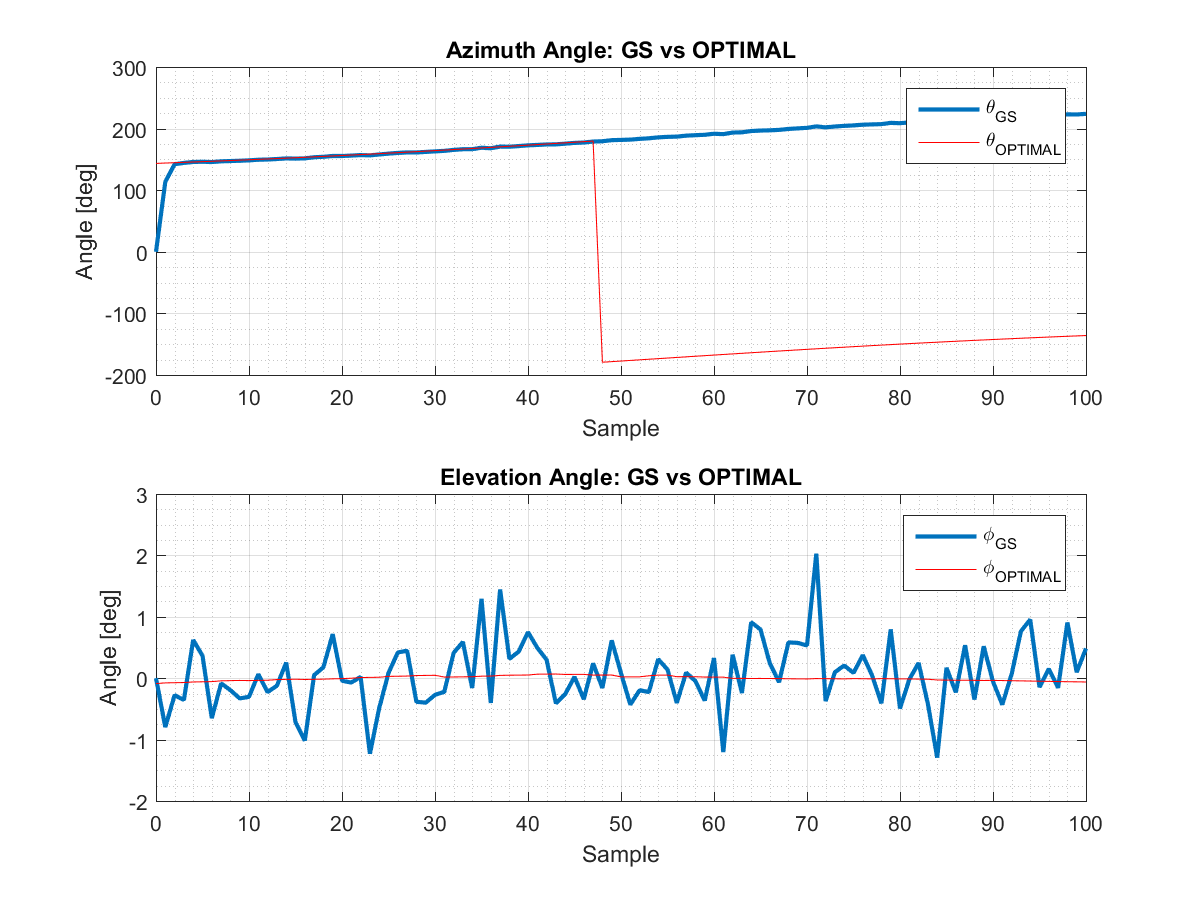
\includegraphics[scale=0.75]{figures/s1_pd_gs.png}
	\caption{Behaviour of the azimuth and elevation angles of the antenna in the GS during the movement of the UA}
	\label{fig:s1_pd_gs_alone}
\end{figure}

The previous explanation describes generally how the angles of the antennas change during the flight of the UA, taking into account the azimuth and elevation angles. However, there are some details related to the response that depend on the type of P-I-D controllers that is applied in the system. Figure \ref{fig:s1_gs} represents the behaviour of P, PI, PD and PID controllers for the given scenario.

Based on the previous simulations of the controllers described on section \ref{sec:controller} and on the azimuthal plots of Figure \ref{fig:s1_gs}, it is possible to verify that the PI and PID controllers have an overshoot, while the P and PD follow directly the desired response. The integral term in the PI and PID controllers is the one responsible for the overshoots due to the accumulation of the error during the whole process. On the other hand, the PID controller is faster than the PI controller because the damping effect of the derivative term attenuates the changes, making the response faster.

In this project, P and PD controllers are not affected by the overshoot and, furthermore, the PD controller is the fastest one (lowest rise time) due to its derivate component.
Based on the elevation plots of Figure \ref{fig:s1_gs}, it is possible to verify that the optimal responses of the P and PI have the bigger variation of the angle than the PD and PID. The derivative component is responsible for the elimination of the small changes which makes the PD and PID controller less sensitive to them. In other words, the PD and PID controllers will not react to small changes while the P and PI will react.

\begin{figure}[H]
	\hfill
	\subfigure[P Controller]{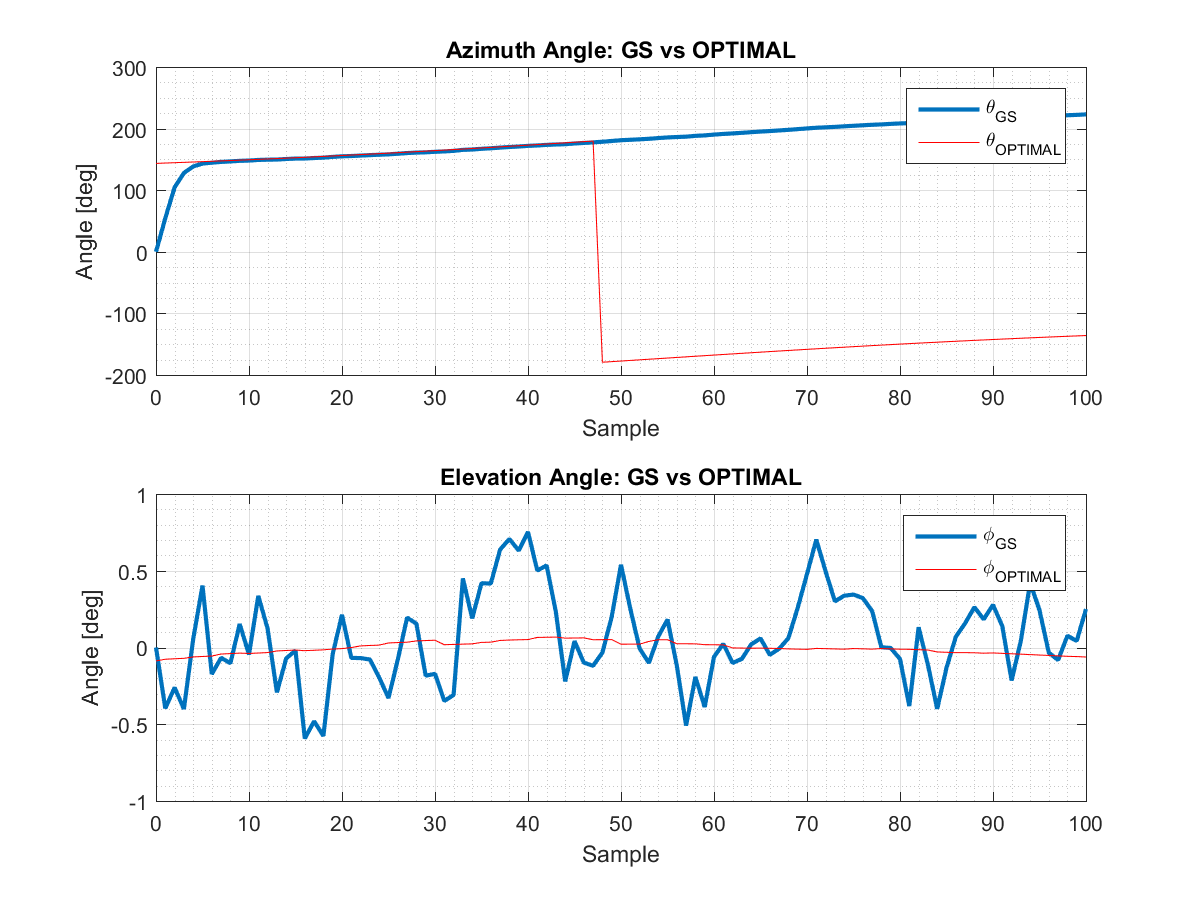
\includegraphics[scale=0.34]{figures/s1_p_gs.png}}
	\hfill
	\subfigure[PI Controller]{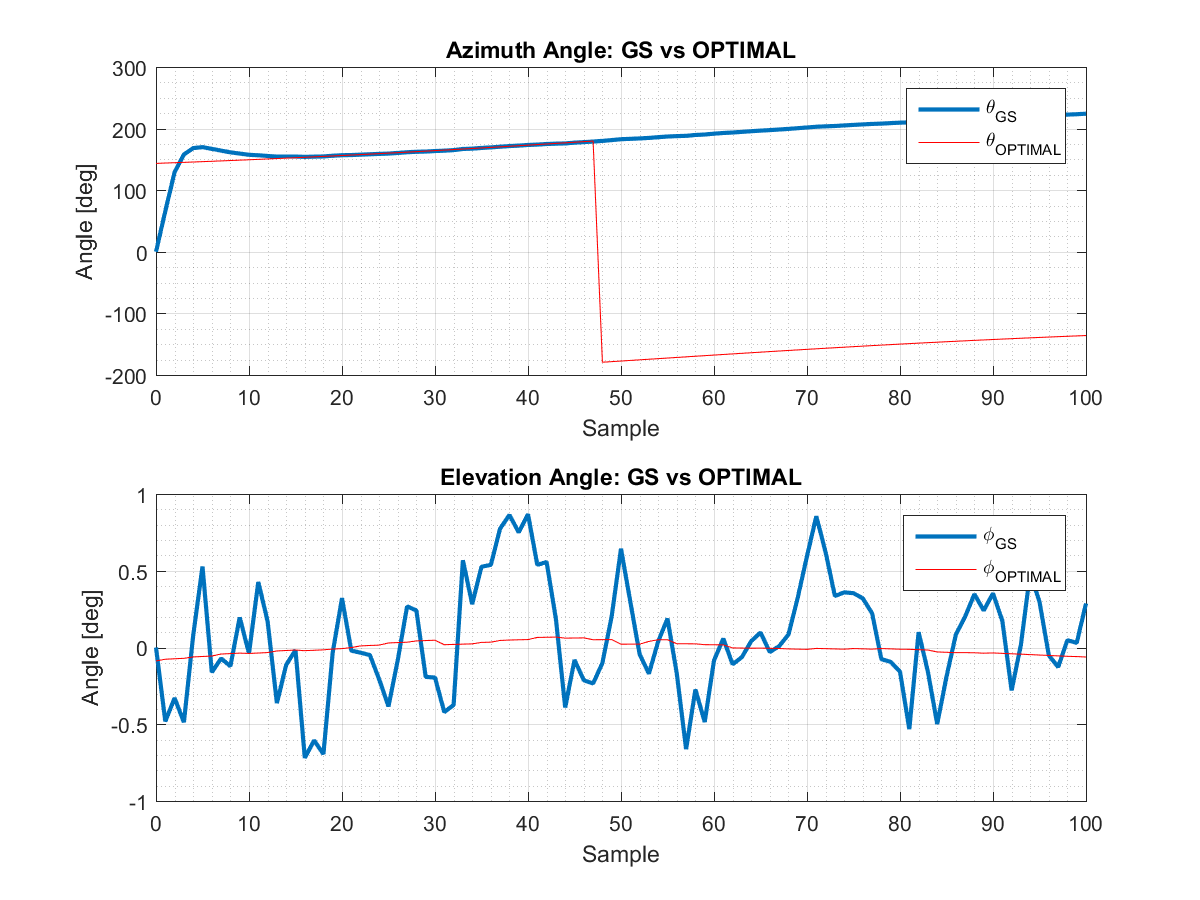
\includegraphics[scale=0.34]{figures/s1_pi_gs.png}}
	\hfill
	\\
	\hfill
	\subfigure[PD Controller]{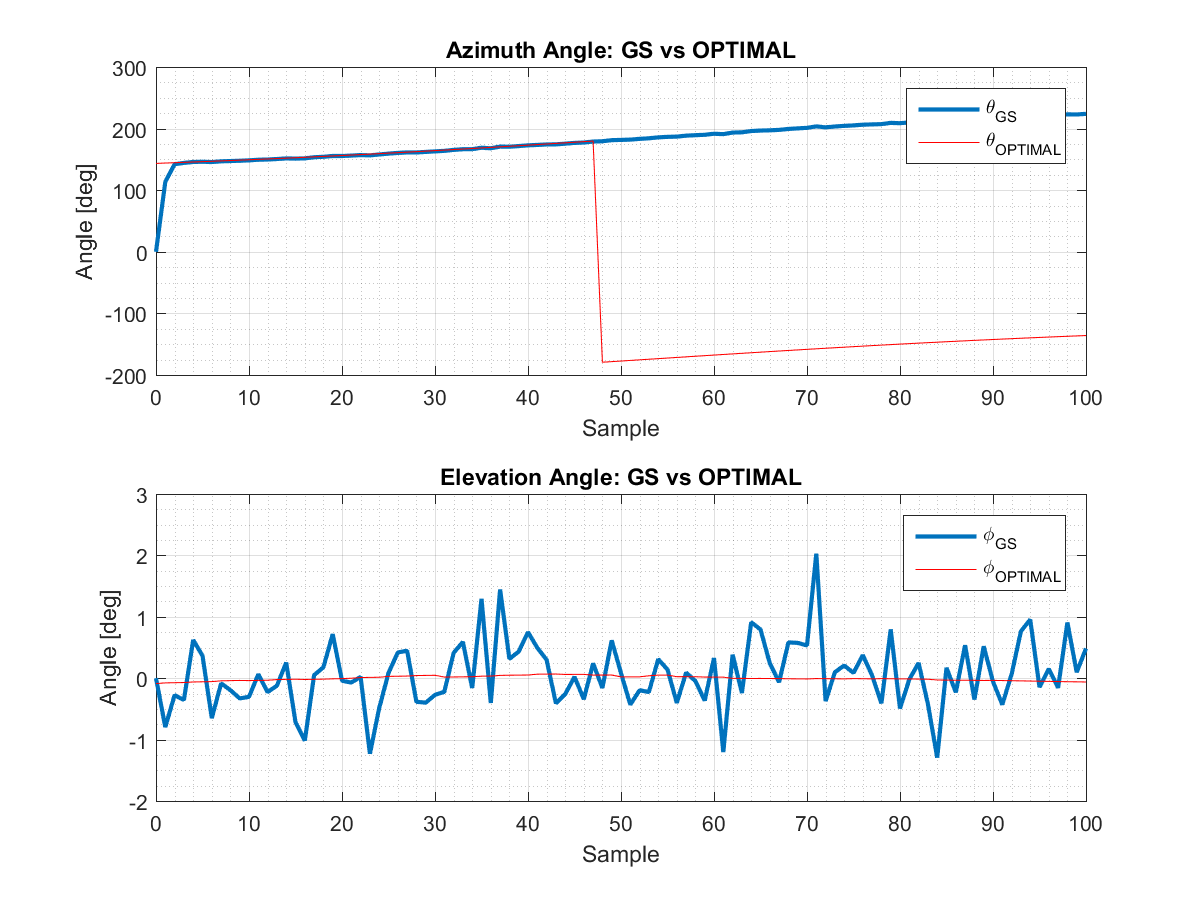
\includegraphics[scale=0.34]{figures/s1_pd_gs.png}}
	\hfill
	\subfigure[PID Controller]{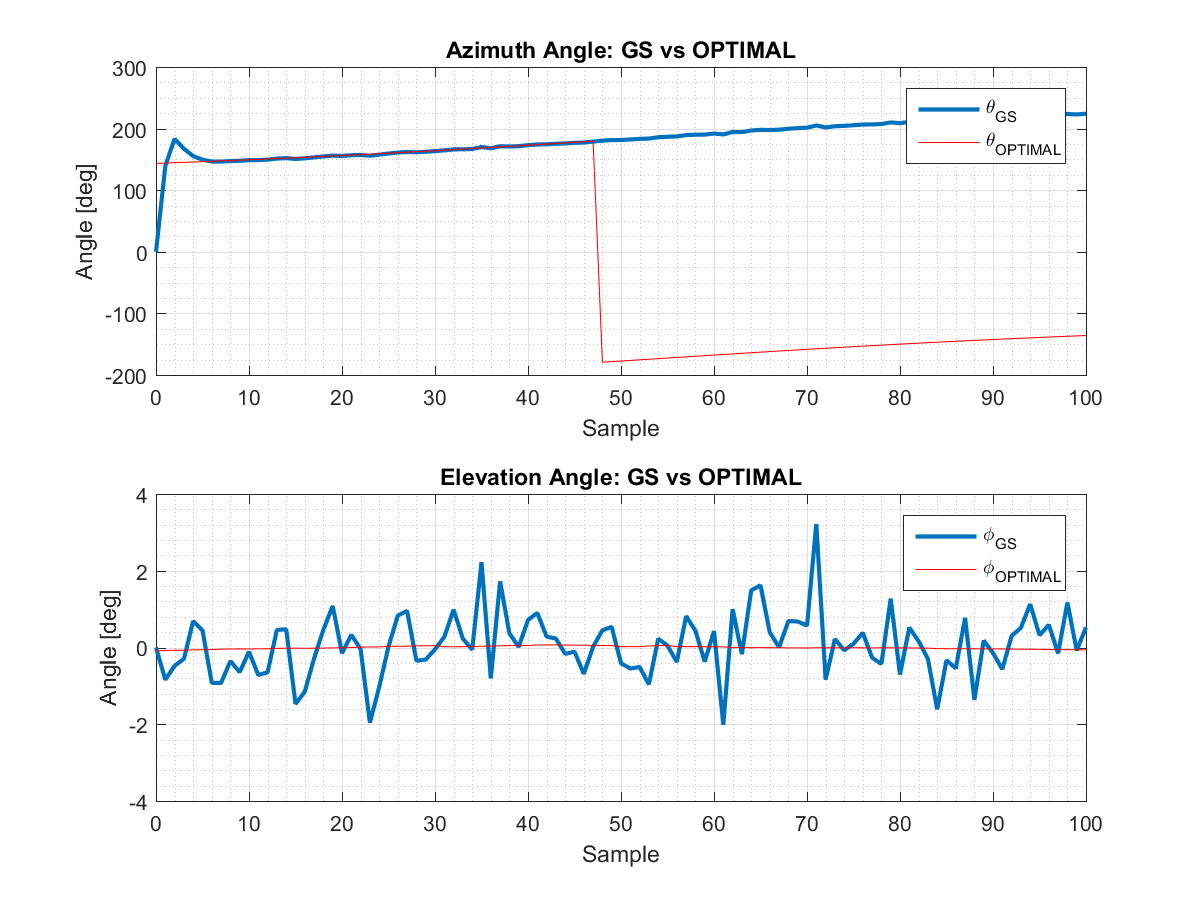
\includegraphics[scale=0.34]{figures/s1_pid_gs.png}}
	\hfill
	\caption{Ground Station controllers}
	\label{fig:s1_gs}
\end{figure}

\subsection{Unmanned Aircraft}
Figure \ref{fig:s1_pd_ua_alone} shows the elevation and azimuth angles of the UA during the whole movement. Based on the fact that the Local NED frame does not coincide with the body frame, it is possible to understand the behaviour of the angle of the antenna. Since the GS is in the right side of the UA (bigger longitude) and the UA is flying towards south (decreasing latitude), the antenna angle will be positive during the whole flight.
The initial $\theta_{OPTIMAL}$ starts around 50 degrees and, as was mentioned before, it increases until around 130 degrees.

The optimal elevation angle, $\phi$, of the UA has almost the same behaviour as the one of the GS. This means that the angle has a small amplitude because there is big distance between the UA and the GS in the second graph of Figure \ref{fig:s1_pd_ua_alone}. Although, in this case, the $\phi_{OPTIMAL}$ has a minimum value instead of a maximum one. This happens because the altitude of the UA is bigger than the one of the GS which demands the antenna to point down.


\begin{figure}[H]
	\centering
	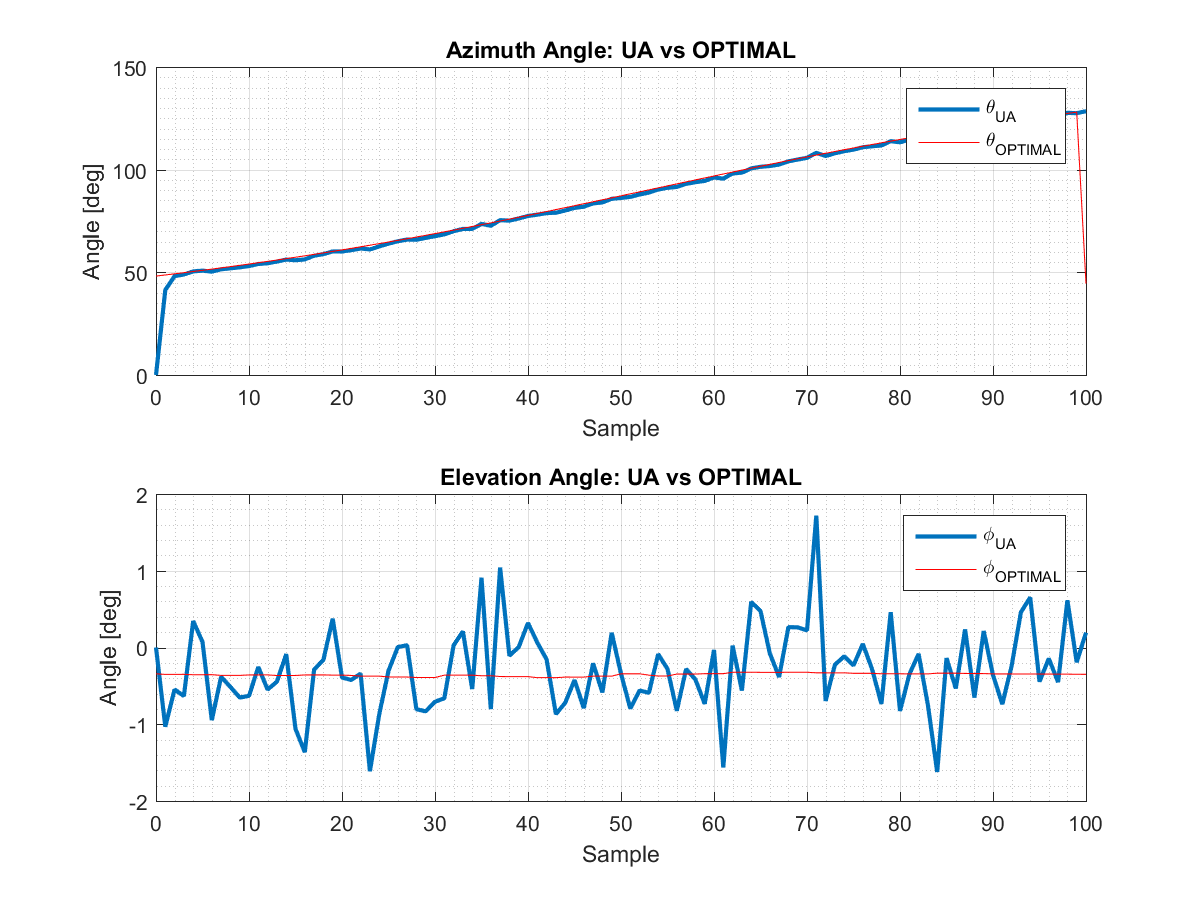
\includegraphics[scale=0.75]{figures/s1_pd_ua.png}
	\caption{Behaviour of the azimuth and elevation angles of the antenna in the UA during its own flight}
	\label{fig:s1_pd_ua_alone}
\end{figure}

The controllers used in this section are the same ones that were used to test the behaviour of the antenna in the GS. This means that the performance will be similar to the ones illustrated in Figure \ref{fig:s1_gs}.

Thus, based on the graphs of the azimuth angle of Figure \ref{fig:s1_ua}, it is observable that the PI and PID controllers have an overshoot when the system is trying to achieve the desired position. Moreover, the response of the sytem with the P and PD controllers achieve directly the desired angle, without any overshoot. On the other hand, the variations of the $\phi$ angle when the system is equipped with a PD or PID controller are less evident than in the P and PI controllers. This is a result of the presence derivative component. In both cases the final results are similar to the ones described in section \ref{GroundStation_scenario1}.

\begin{figure}[H]
	\hfill
	\subfigure[P Controller]{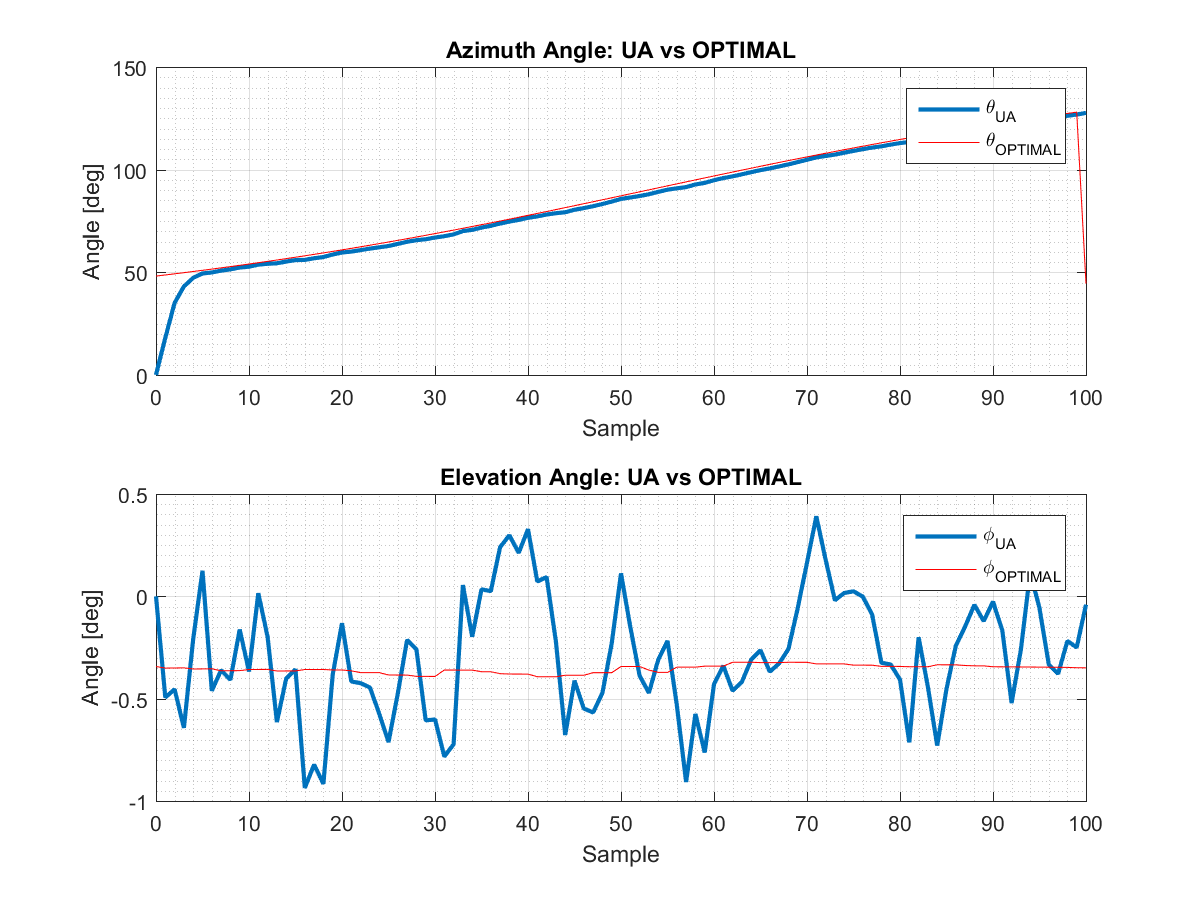
\includegraphics[scale=0.34]{figures/s1_p_ua.png}}
	\hfill
	\subfigure[PI Controller]{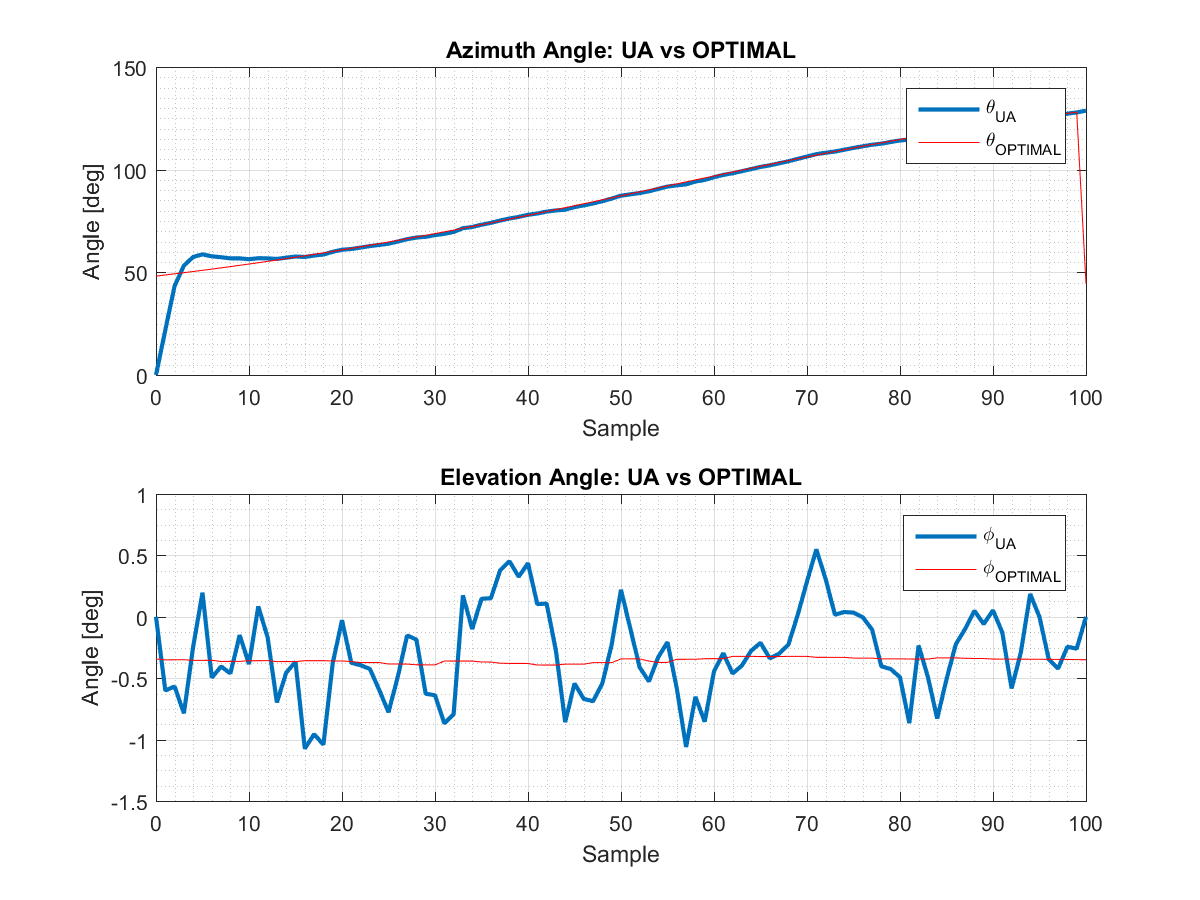
\includegraphics[scale=0.34]{figures/s1_pi_ua.png}}
	\hfill
	\\
	\hfill
	\subfigure[PD Controller]{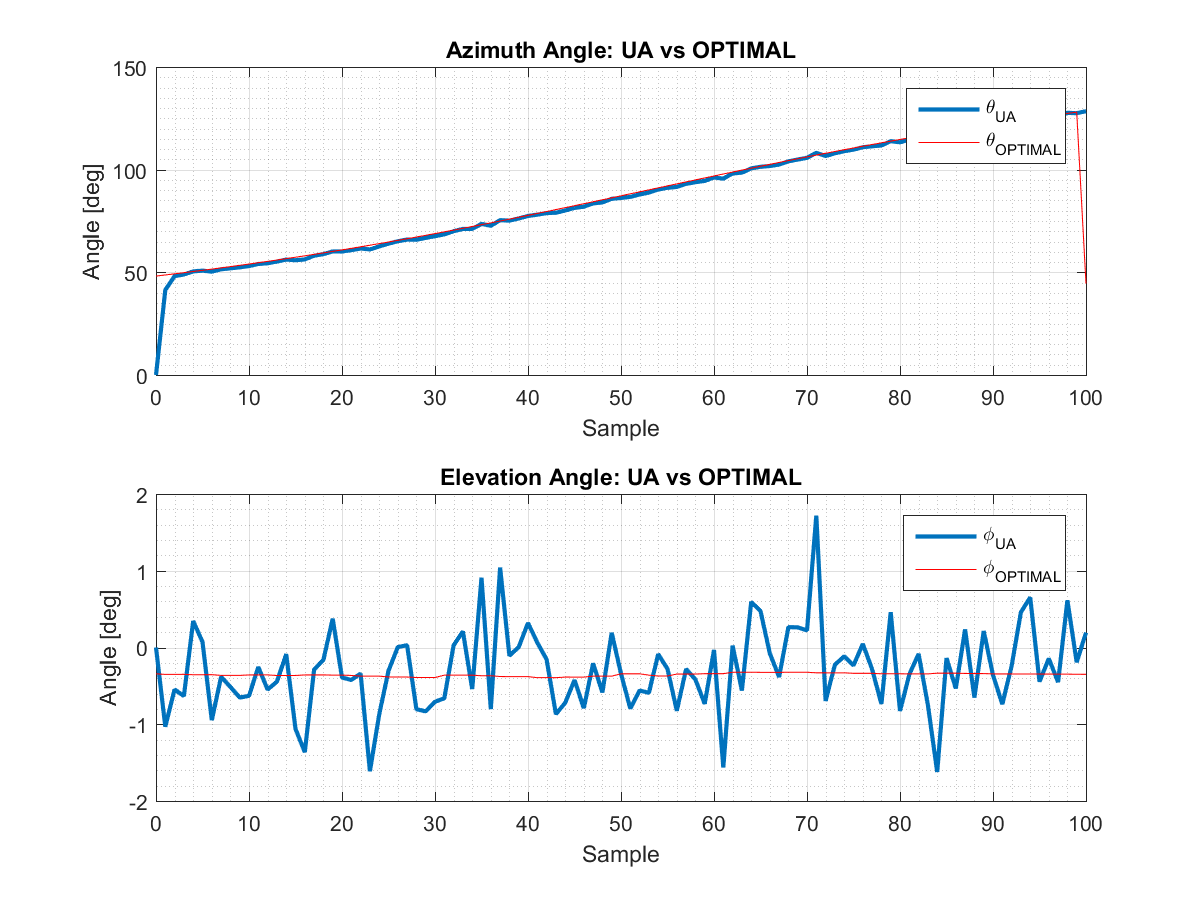
\includegraphics[scale=0.34]{figures/s1_pd_ua.png}}
	\hfill
	\subfigure[PID Controller]{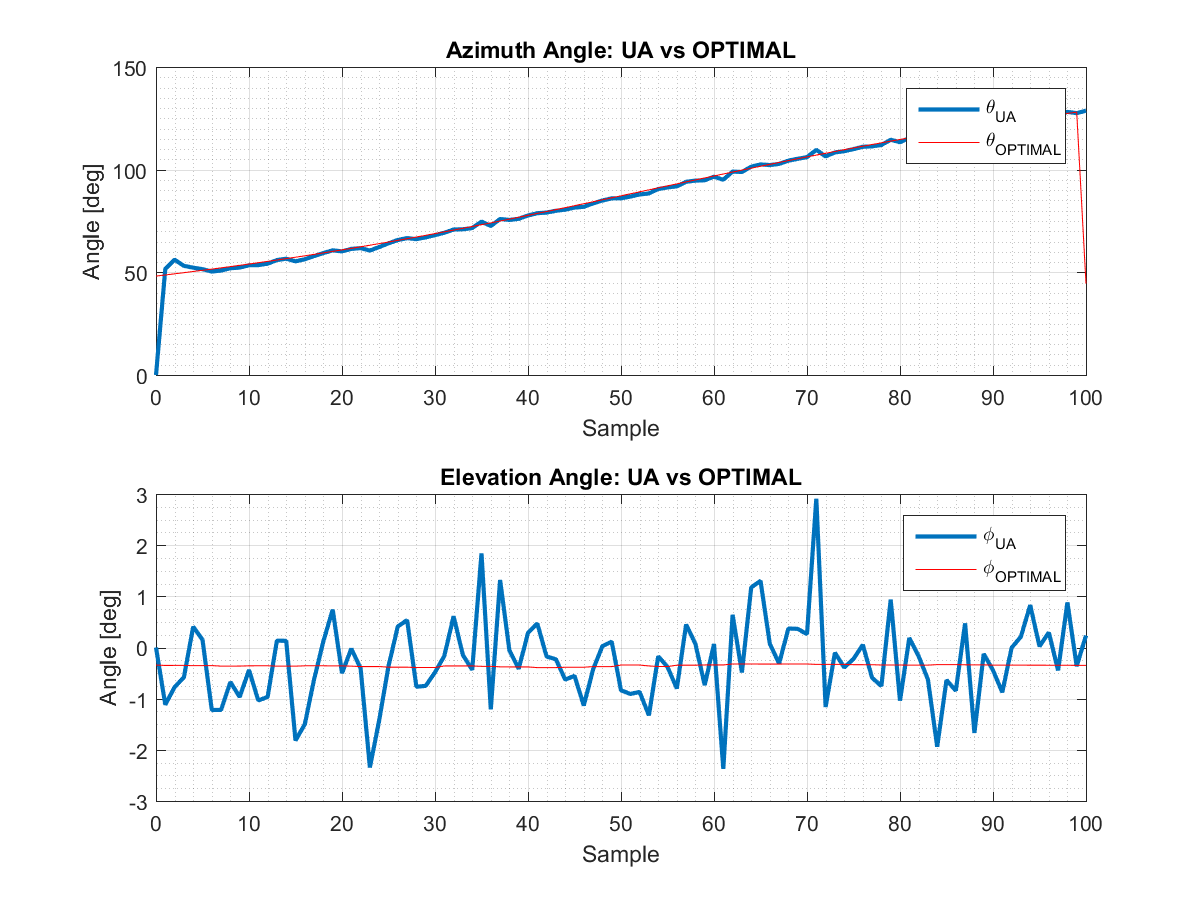
\includegraphics[scale=0.34]{figures/s1_pid_ua.png}}
	\hfill
	\caption{Unmanned Aircraft Controllers}
	\label{fig:s1_ua}
\end{figure}

\subsection{Power}
IDEAS
In Figure \ref{fig:s2_power} the power at the receiver antenna of the GS antenna can be seen.
Power related to the controllers used
Biggest change in the beginning and depends on the controller that is used.
Big overshoot - the power decreases a lot because the antenna goes and comes back.
Without integral component there is no overshoot so the difference between them is only the time that they need ti achieve the perfect angle.


\begin{figure}[H]
	\hfill
	\subfigure[P]{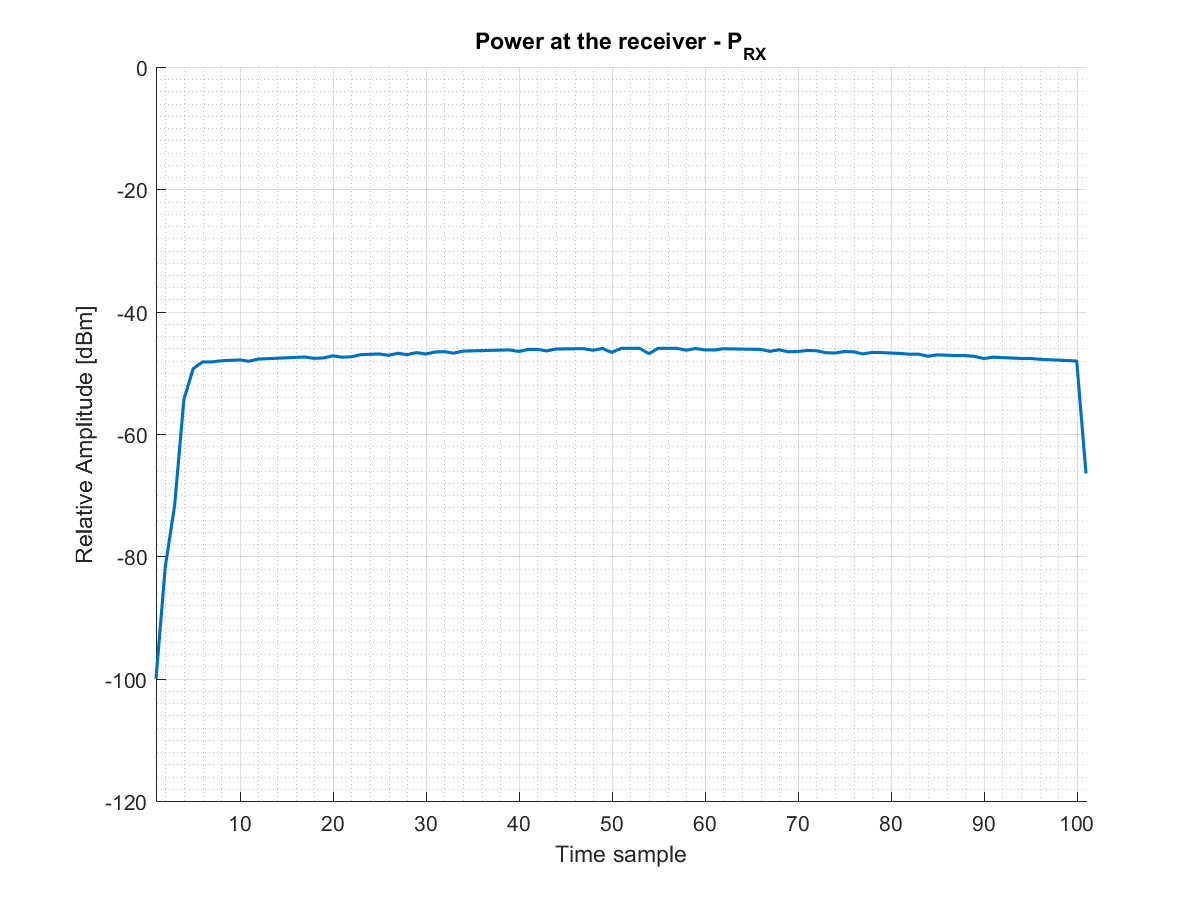
\includegraphics[scale=0.34]{figures/s1_p_power.png}}
	\hfill
	\subfigure[PI]{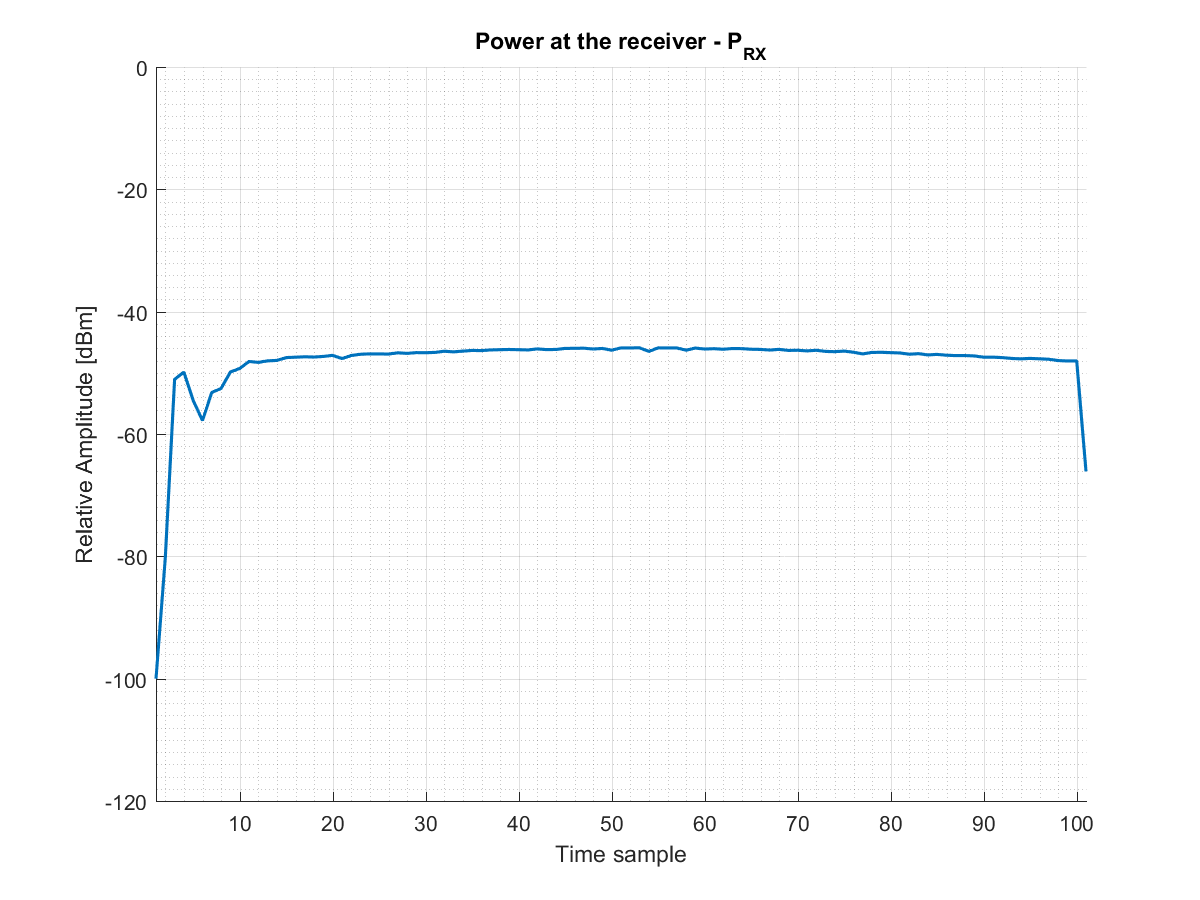
\includegraphics[scale=0.34]{figures/s1_pi_power.png}}
	\hfill
	\\
	\hfill
	\subfigure[PD]{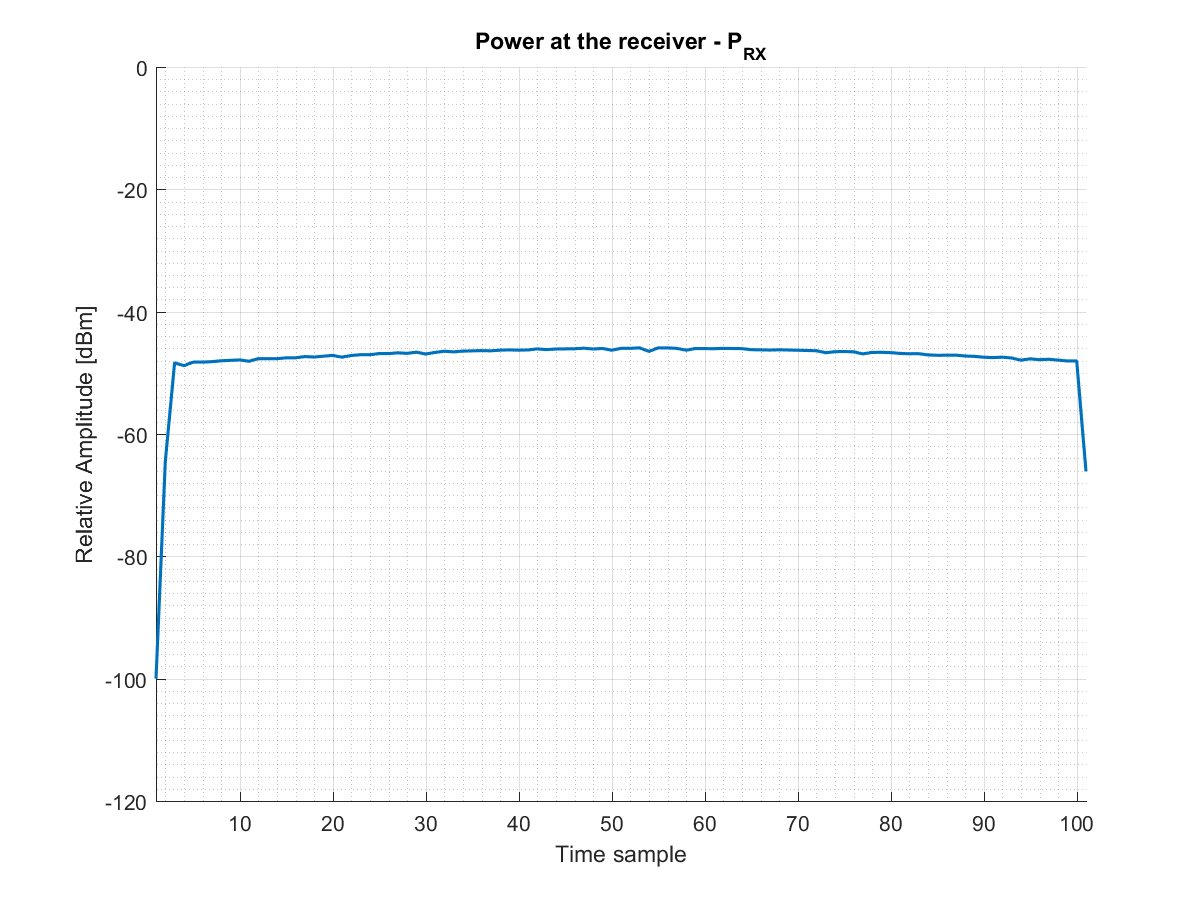
\includegraphics[scale=0.34]{figures/s1_pd_power.png}}
	\hfill
	\subfigure[PID]{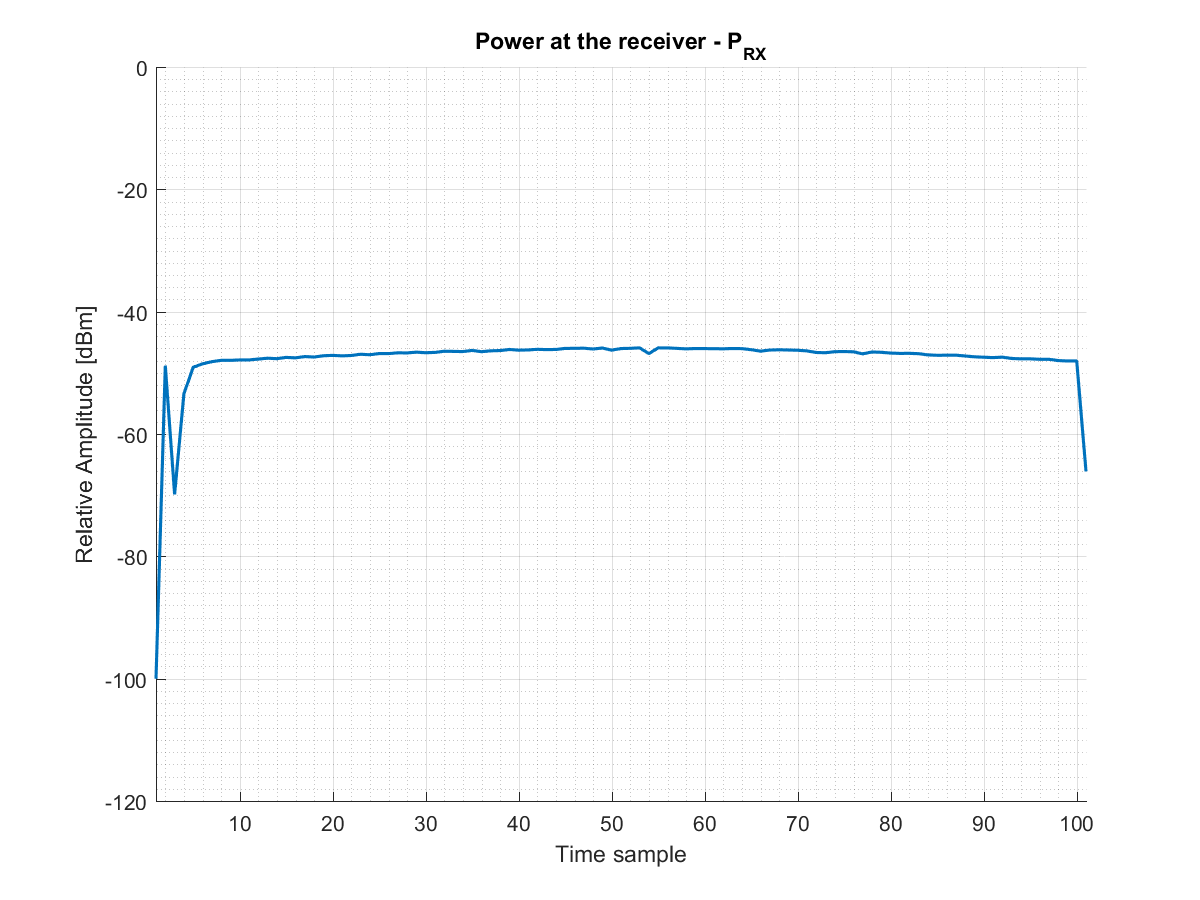
\includegraphics[scale=0.34]{figures/s1_pid_power.png}}
	\hfill
	\caption{UA Controllers}
	\label{fig:s1_power}
\end{figure}
